% !TeX spellcheck = en_GB
% !TeX program = lualatex
%
% v 2.3  Feb 2019   Volker RW Schaa
%		# changes in the collaboration therefore updated file "jacow-collaboration.tex"
%		# all References with DOIs have their period/full stop before the DOI (after pp. or year)
%		# in the author/affiliation block all ZIP codes in square brackets removed as it was not %         understood as optional parameter and ZIP codes had bin put in brackets
%       # References to the current IPAC are changed to "IPAC'19, Melbourne, Australia"
%       # font for ‘url’ style changed to ‘newtxtt’ as it is easier to distinguish "O" and "0"
%
\documentclass[a4paper,
               %boxit,        % check whether paper is inside correct margins
               %titlepage,    % separate title page
               %refpage       % separate references
               %biblatex,     % biblatex is used
               keeplastbox,   % flushend option: not to un-indent last line in References
               %nospread,     % flushend option: do not fill with whitespace to balance columns
               %hyphens,      % allow \url to hyphenate at "-" (hyphens)
               %xetex,        % use XeLaTeX to process the file
               %luatex,       % use LuaLaTeX to process the file
               ]{jacow}
%
% ONLY FOR \footnote in table/tabular
%
\usepackage{pdfpages,multirow,ragged2e} %
\usepackage{tablefootnote}
%
% CHANGE SEQUENCE OF GRAPHICS EXTENSION TO BE EMBEDDED
% ----------------------------------------------------
% test for XeTeX where the sequence is by default eps-> pdf, jpg, png, pdf, ...
%    and the JACoW template provides JACpic2v3.eps and JACpic2v3.jpg which
%    might generates errors, therefore PNG and JPG first
%
\makeatletter%
	\ifboolexpr{bool{xetex}}
	 {\renewcommand{\Gin@extensions}{.pdf,%
	                    .png,.jpg,.bmp,.pict,.tif,.psd,.mac,.sga,.tga,.gif,%
	                    .eps,.ps,%
	                    }}{}
\makeatother
\newcommand{\ts}{\textsuperscript}
% CHECK FOR XeTeX/LuaTeX BEFORE DEFINING AN INPUT ENCODING
% --------------------------------------------------------
%   utf8  is default for XeTeX/LuaTeX
%   utf8  in LaTeX only realises a small portion of codes
%
\ifboolexpr{bool{xetex} or bool{luatex}} % test for XeTeX/LuaTeX
 {}                                      % input encoding is utf8 by default
 {\usepackage[utf8]{inputenc}}           % switch to utf8

\usepackage[USenglish]{babel}
\usepackage{subcaption}

%
% if BibLaTeX is used
%
\ifboolexpr{bool{jacowbiblatex}}%
 {%
  \addbibresource{jacow-test.bib}
  \addbibresource{biblatex-examples.bib}
 }{}
\listfiles

%%
%%   Lengths for the spaces in the title
%%   \setlength\titleblockstartskip{..}  %before title, default 3pt
%%   \setlength\titleblockmiddleskip{..} %between title + author, default 1em
%%   \setlength\titleblockendskip{..}    %afterauthor, default 1em

\begin{document}

\title{Comissionamento do Wiggler W180}

\author{Envolvidos: Liu Lin, Ximenes Resende, Murilo Alves \\ FAC - LNLS \\ Segunda-feira, 19 de setembro de 2022}
\maketitle
%
\section{Resumo}
Primeiras caracterizações do efeito do wiggler W180 no feixe do anel de armazenamento. Foram medidas as distorções de órbita em cada gap. Chegamos no gap de \SI{49.73}{\milli\meter} que corresponde ao campo de \SI{1}{\tesla}, medimos a matriz resposta de órbita das corretoras do wiggler e corrigimos a órbita o melhor possível com estas corretoras. Depois disto fizemos uma análise LOCO neste gap e aplicamos correções da ordem de \SI{-1}{\percent} nos quadrupolos QDB2 próximos ao wiggler para corrigir efeitos de gradiente. O acoplamento medido foi de \SI{1.5}{\percent}, \SI{0.5}{\percent} acima do valor que normalmente operamos. Corrigimos o acoplamento para zero e depois subimos para \SI{1}{\percent} com os quadrupolos skew acromáticos. A eficiência de injeção típica com gap do wiggler em \SI{49.73}{\milli\meter} foi de \SI{80}{\percent} sem otimizações do sistema injetor. Depois destas caracterizações iniciais disponibilizamos a máquina para condicionamento do vácuo das linhas de luz. 

\section{Distorções de órbita}
Registramos a órbita com o gap do wiggler aberto em \SI{300}{\milli\meter} e em seguida as distorções de órbita conforme se reduzia o gap até o valor de \SI{49.73}{\milli\meter}, correspondente a \SI{1}{\tesla}. A Figura~\ref{fig:dist1} mostra a distorção de órbita horizontal e vertical ao longo do anel para cada gap, conforme indicado pela legenda. Na Figura~\ref{fig:dist2} estão representados os valores pico-a-pico das distorções apresentadas na Figura~\ref{fig:dist1} em função do gap do wiggler. Observa-se que a maior distorção horizontal e vertical ocorre no gap \SI{70}{\milli\meter}.
\begin{figure*}[!h]
    \centering
    \includegraphics*[width=\textwidth]{orbit_distortion_gap_wiggler.png}
    \caption{Distorção de órbita medida em relação a órbita com gap de \SI{300}{\milli\meter}.}
    \label{fig:dist1}
\end{figure*}
\begin{figure*}[!h]
    \centering
    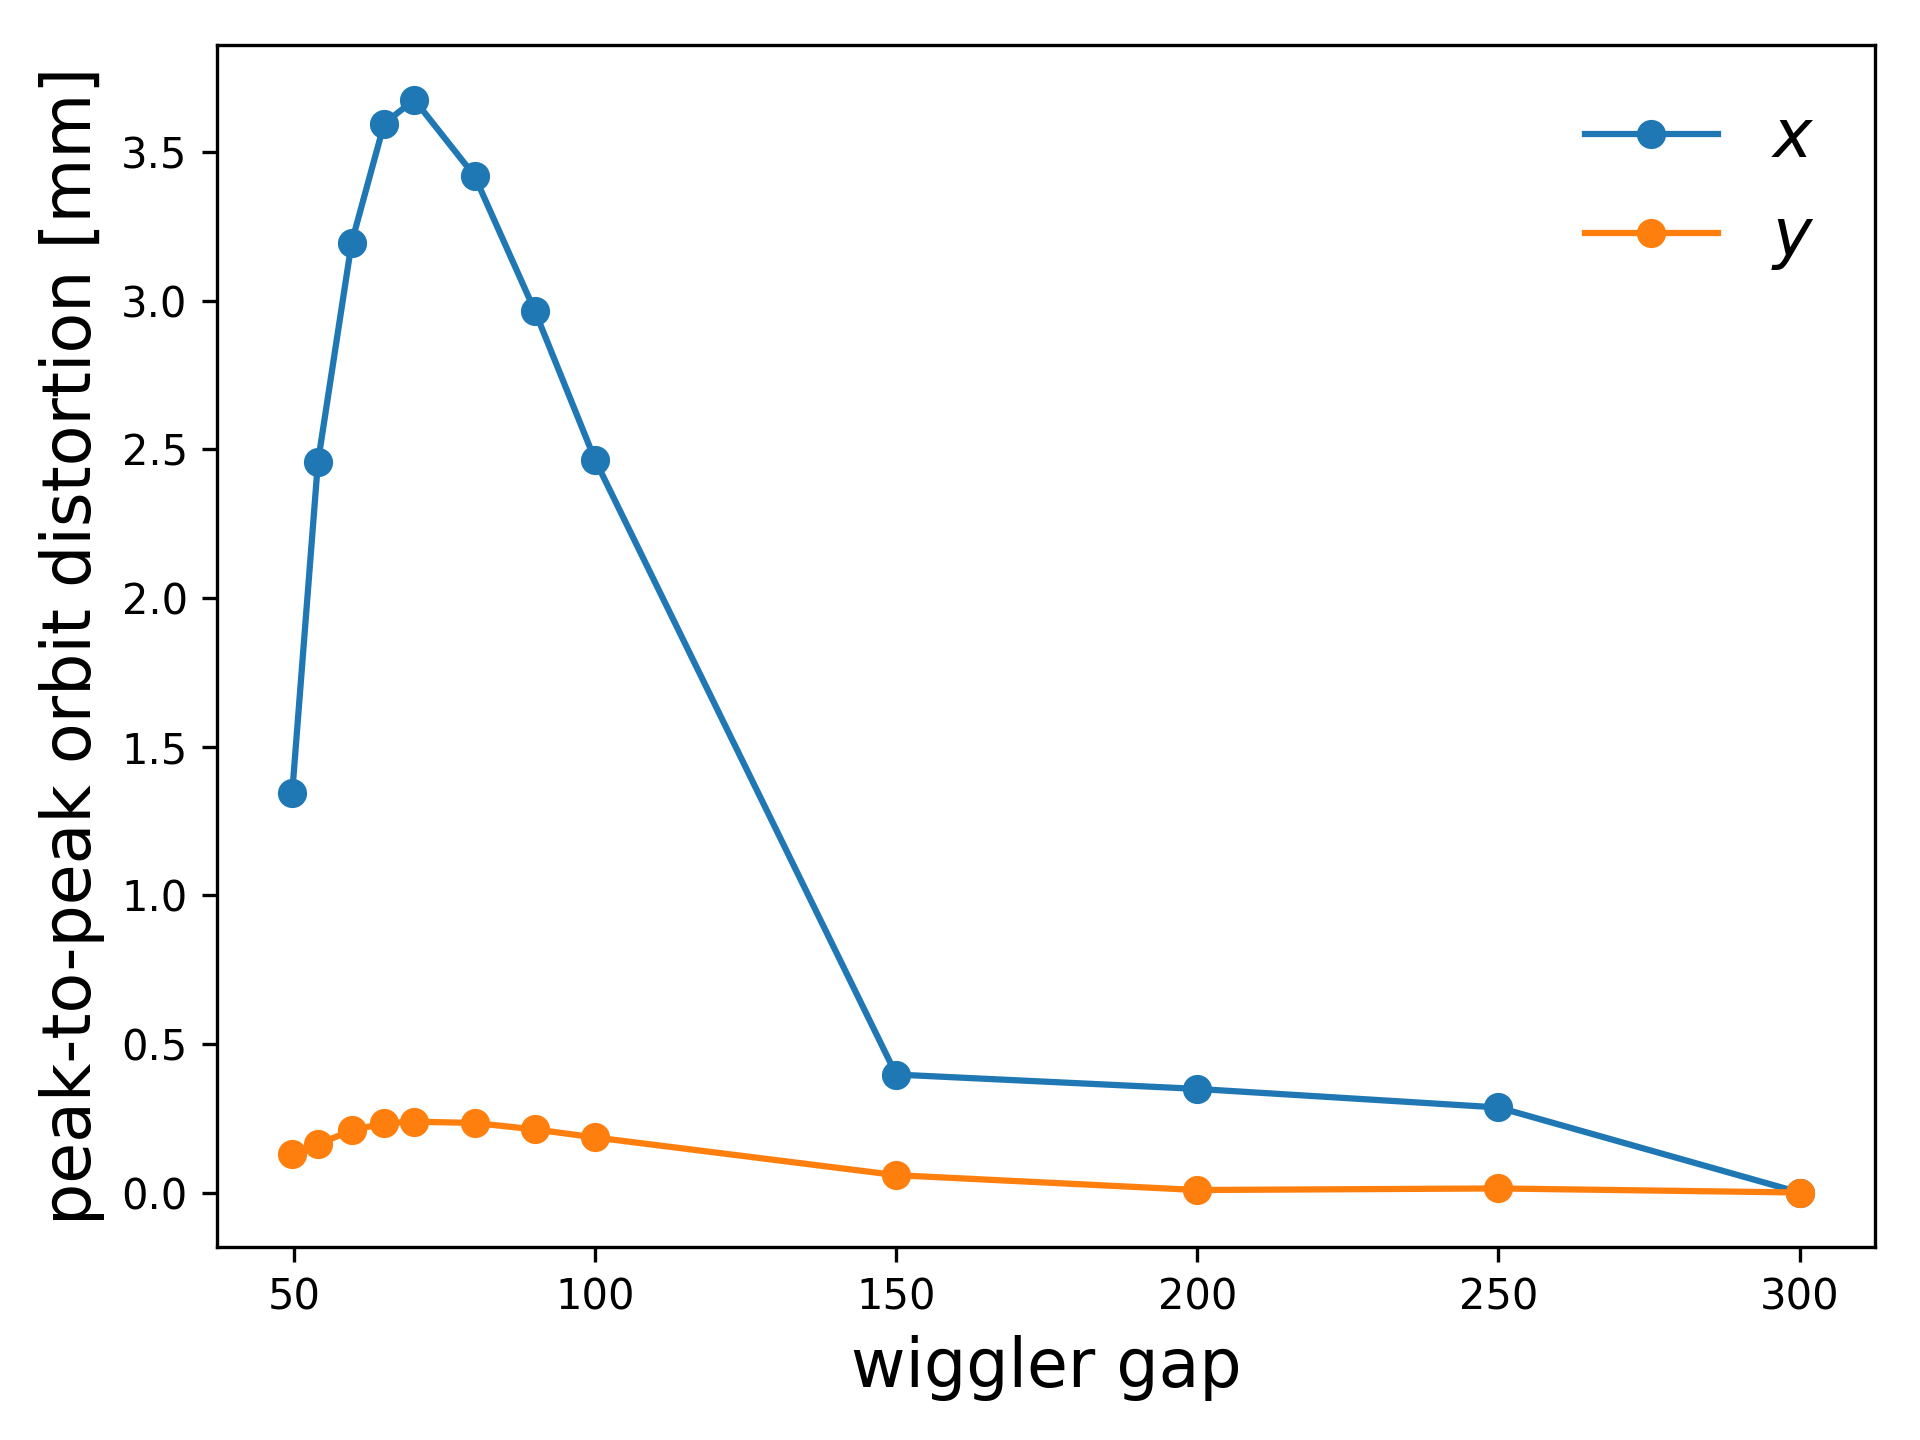
\includegraphics[width=0.75\textwidth]{orbit_distortion_ptp_vs_gap_wiggler.png}
    \caption{Distorção pico-a-pico em função do gap do wiggler}
    \label{fig:dist2}
\end{figure*}

\section{Matriz resposta de correção local de órbita}
Para o gap de \SI{49.73}{\milli\meter}, aplicamos as correntes $+\SI{1.0}{\ampere}$ na corretora SI-14SB:PS-CH-1 (upstream) e \SI{-0.9}{\ampere} na corretora SI-14SB:PS-CH-2 (downstream). Este foram os valores obtidos para corrigir primeira e segunda integral do wiggler medidas em bancada. Porém estas correções não resultaram em uma boa correção da distorção de órbita gerada pelo wiggler. Em torno deste ponto, corrigimos a órbita com o SOFB mesmo e medimos a matriz resposta de órbita destas corretoras do wiggler. As assinaturas desta matriz, em unidades de \SI{}{\micro\meter/\ampere}, estão apresentadas na Figura~\ref{fig:respmat}.
\begin{figure*}
    \centering
    \includegraphics*[width=0.9\textwidth]{respmat_gap49p73mm_Iup_pos1p0A_Idown_neg0p9.png}
    \caption{Matriz resposta de órbita medida. Até o índice 160 temos medidas horizontais e de 160 até 320 temos as medidas verticais.}
    \label{fig:respmat}
\end{figure*}

A partir desta matriz de correção de órbita, calculamos que para corrigir a distorção de órbita entre gap \SI{49.73}{\milli\meter} e \SI{300}{\milli\meter}, as correntes das corretoras deveriam ser $+\SI{1.96}{\ampere}$ (upstream) e $\SI{-1.0}{\ampere}$ (downstream), ou seja, a corretora upstream deveria ter uma corrente quase duas vezes maior para corrigir a distorção de órbita. Removemos as correções com o SOFB e aplicamos as correntes mencionadas nas corretoras ao redor do wiggler. A distorção de órbita reduziu consideravelmente com estas correntes. Guiado pelos kicks calculados pelo SOFB para corrigir o resíduo de órbita, variamos as correntes destas corretoras em torno do valor calculado, obtendo que as correntes $I_{\mathrm{CH1}}=+\SI{1.4973}{\ampere}$ e $I_{\mathrm{CH2}}=\SI{-1.1706}{\ampere}$ reduziram o resíduo de órbita para um rms $<\SI{10}{\micro\meter}$ na horizontal.
\section{Correção de ótica e acoplamento com LOCO}
Com o gap do wiggler em $\SI{49.73}{\milli\meter}$ e as corretoras em $I_{\mathrm{CH1}}=+\SI{1.4973}{\ampere}$ e $I_{\mathrm{CH2}}=\SI{-1.1706}{\ampere}$ para corrigir a distorção de órbita, corrigimos o resíduo com o SOFB e medimos uma matriz resposta de correção global de órbita para fazer a análise LOCO. A partir da calibração desta matriz, obtivemos as forças de quadrupolos apresentadas na Figura~\ref{fig:quad}. Fica claro uma variação maior nos quadrupolos QDB2 do trecho 14, indicando a necessidade de compensar efeitos de gradiente de campo gerados pelo wiggler. O betabeating indicado por esse modelo calibrado foi menor que \SI{2}{\percent} para ambos os planos. 
\begin{figure*}
    \centering
    \includegraphics*[width=0.9\textwidth]{trimquads_correction_W180_iter0.png}
    \caption{Oposto das correções de ótica calculadas pelo LOCO}
    \label{fig:quad}
\end{figure*}

Também medimos a separação mínima de sintonias, indicando que o wiggler aumentou o acoplamento global da máquina em~\SI{0.5}{\percent}, como pode ser visto no gráfico da esquerda da Figura~\ref{fig:coup}. Também observamos que os termos fora da diagonal da matriz resposta também aumentaram, indicando aumento de acoplamento local. Aplicamos as variações de forças nos quadrupolos normais indicados na Figura~\ref{fig:quad} e também os quadrupolos skew para zerar o acoplamento. Em seguida medimos a separação mínima de sintonias, resultando em um valor muito próximo de zero, como apresenta o gráfico central da Figura~\ref{fig:coup}. Após isso, alteramos os quadrupolos skew acromáticos para subir o acoplamento global para \SI{1}{\percent}, valor que definimos para ser de operação. O resultado da medida de acoplamento após este procedimento está no gráfico da direita na Figura~\ref{fig:coup}.
\begin{figure*}
    \centering
    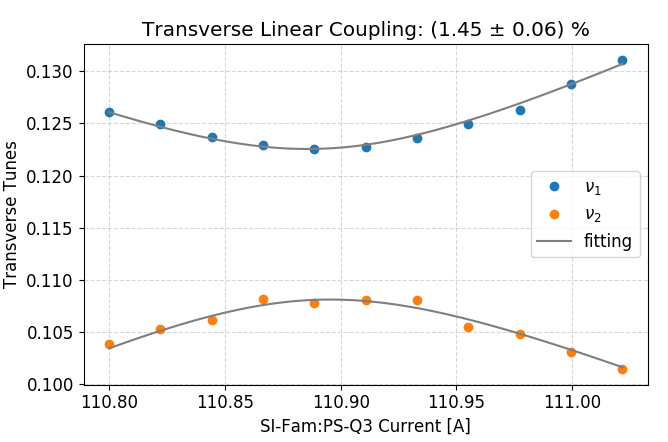
\includegraphics[width=0.33\textwidth]{coupling_W180_n01.png}
    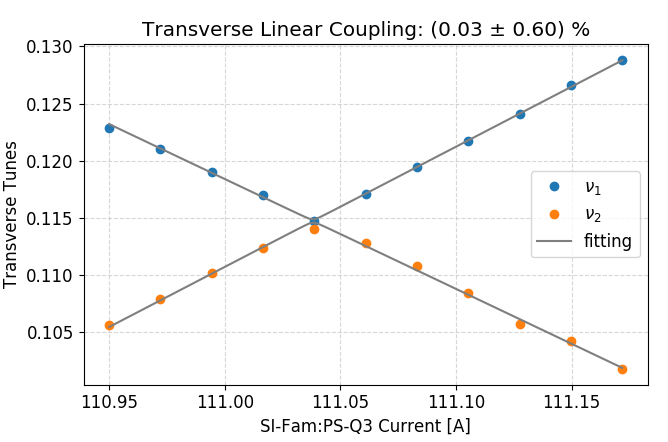
\includegraphics[width=0.33\textwidth]{coupling_W180_n01_coup_corr.png}
    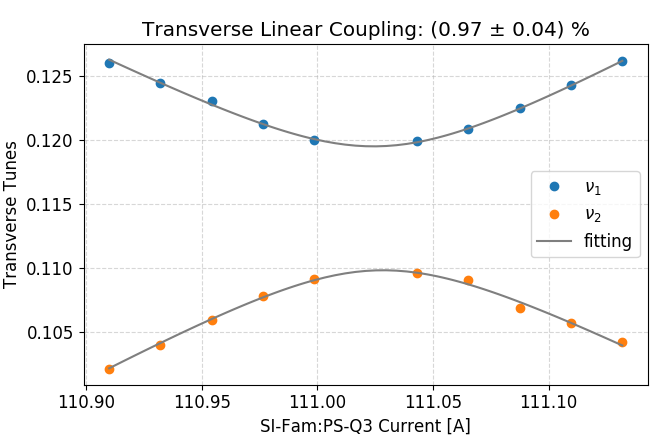
\includegraphics[width=0.33\textwidth]{coupling_W180_n01_coup_corr_to_1pc.png}
    \caption{Medida de acoplamento. Antes da correção (esquerda), depois da correção (meio), depois de aumentar para \SI{1}{\percent} (direita).}
    \label{fig:coup}
\end{figure*}

Após essas correções de órbita, ótica e acoplamento, testamos a injeção (sem otimizar posição e ângulo) e obtivemos eficiência de injeção no anel típica de \SI{80}{\percent}.

\section{Conclusões}
Caracterizamos parcialmente alguns efeitos do wiggler W180 instalado no anel na parada de Setembro/2022. Medimos as distorções de órbita para alguns gaps e dedicamos um pouco mais de tempo para medidas com gap de~\SI{49.73}{\milli\meter}, correspondente ao campo de \SI{1}{\tesla}. Encontramos as correntes das corretoras dedicadas ao wiggler para corrigir a distorção de órbita introduzida pelo ID. Foi necessário aplicar correntes diferentes do esperado pelas medidas em bancada nas corretoras do wiggler para corrigir a distorção de órbita. Identificamos perturbações na ótica devido ao wiggler e corrigimos com as trimcoils dos quadrupolos, a maior variação se deu alterando as forças dos quadrupolos QDB2 em torno do wiggler da ordem de \SI{1}{\percent}. Observamos que o wiggler introduziu acoplamento na máquina, mas foi possível corrigir para próximo de zero com os quadrupolos skew da máquina. Depois disso subimos o acoplamento global para \SI{1}{\percent} e observamos boa eficiência de injeção mesmo sem otimizar o sistema injetor. Uma configuração global com as correções foi salva. Em seguida, disponibilizamos a máquina para condicionamento de vácuo das linhas de luz. Mais caracterizações mais sistemáticas serão feitas ao longo dos próximos estudos de máquina.

\end{document}
